

\chapter{Introduction}

This dissertation thesis contributes to the research field of crowd management from the perspective of a computer scientist: I design and test a novel crowd guidance system in which crowds are redirected by employing direct communication technology. The contributions are:
\begin{itemize}
\item A \textbf{proof of concept of the design} of a system in which crowds are redirected through mobile applications based on direct communication.
\item A \textbf{methodology} how such a system can be developed systematically by combining models and methods from engineering, psychology, and computer science.
\item A \textbf{simulation framework} with which such a system can be investigated (collaboratively developed in the \textit{roVer} research project work).
\end{itemize}


\vspace{0.4cm}

\tcbset{colback=gray!5!white,colframe=gray!50!black,fonttitle=\bfseries}
\begin{tcolorbox}[title=Availability of data and software]
This work is based on the principles of Open Science. Source code and data, including raw data, are freely available. Parts of the software that were developed in collaboration are clearly reported. See Appendix~\ref{sec:availability}.
\end{tcolorbox}

\section{Motivation}

Despite numerous efforts to increase the safety of crowds, crowd crushes still occur~\cite{haghani-2018-cdyn}. In 2022, 159 people died in the Seoul accident on Halloween. In 2023, 12 people died at a soccer match in El Salvador. More than 2000 people died during the Mina stampede in 2015. In Europe, the Love Parade (2010) and the Oxford Circus stampede (2017) are among the best-known crowd crushes of recent years. 
However, crowds of people gather not only at large events but also in everyday life. In large cities, this mainly affects local public transport. With growing urbanization, transport hubs are becoming increasingly congested, which will be further exacerbated by efforts to reduce vehicle traffic in cities. Consequently, numerous cities declared their goal to make pedestrian traffic safer and more comfortable: London launched the Walking Action Plan of London in 2018, Munich released a Mobility Strategy in 2019, and Berlin declared the Mobility Act in 2021.  
To achieve this, new traffic strategies for pedestrians and crowds are needed.

%(\url{https://content.tfl.gov.uk/mts-walking-action-plan.pdf}), 
 %~(\url{https://www.muenchen-transparent.de/dokumente/7454207}) (\url{https://www.berlin.de/sen/uvk/mobilitaet-und-verkehr/verkehrspolitik/mobilitaetsgesetz/})}.

One step towards making traffic safer is to provide safety-relevant information to crowds. To distribute the information, crowd managers typically use signs, light signals, loudspeaker announcements, or employ staff on site. Another approach is to inform the crowd through mobile applications. This, however, requires that information is reliably disseminated over the mobile network.
At events with large crowds, the cellular network is often overloaded, which poses the risk that safety-relevant information is lost. One idea is to employ direct communication technologies where data is exchanged directly from device to device, see Fig.~\ref{fig:scenarios}.
With this, safety-relevant information could be provided to the crowd independently of the network infrastructure, which is crucial in emergencies. 


\begin{figure}[hbt!]
\centering
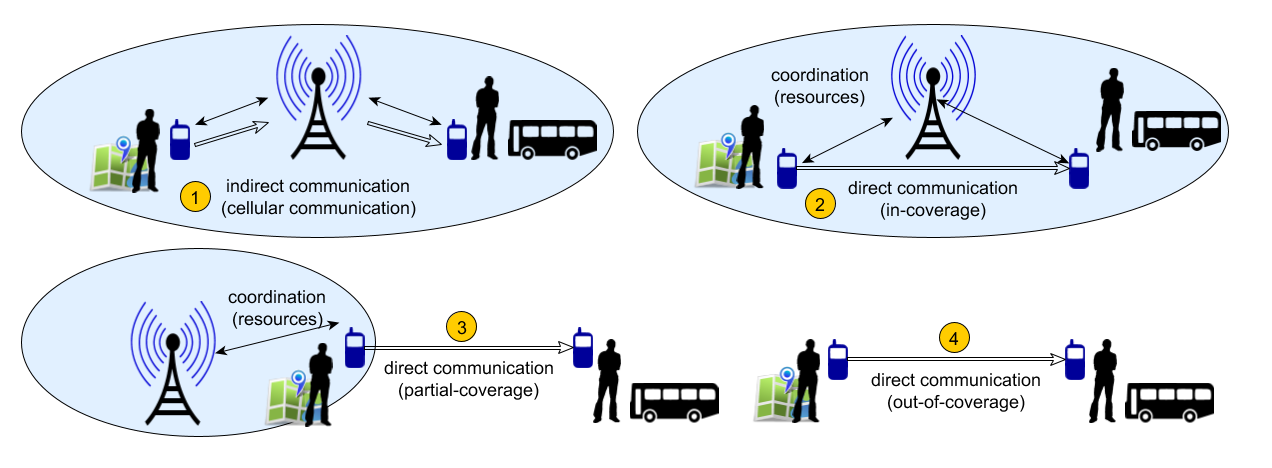
\includegraphics[width=14cm,trim={0 0.5cm 0 0.5cm},clip]{./introduction/directCommunication.png} 
\caption[Cellular communication]{Direct communication in cellular networks. Devices share data via the base station~(1). With direct communication, devices share data directly~(2). Communication is possible even in partial coverage (3) or out-of-coverage (4) scenarios. Usage of the graphic granted by the creator.}
\label{fig:scenarios}
\end{figure}



Direct communication is specified in several mobile standards, whereby two primary technologies have emerged. The first is dedicated short range communication, which is based on WLAN ad hoc networks~\cite{stanley-2023-com}. The first standard was published in 2010 and amended in 2023. The second is `cellular vehicle-to-everything' (C-V2X) communication, which has been developed since the 2010s, gaining more attention through the transition to 5G~\cite{anwar-2019-com}. 
The initial focus of both technologies was on vehicle communication.
However, vehicle and pedestrian traffic differ strongly: People do not move in lanes, their speed is lower, and they can be closer to each other than cars. 
For this reason, 
the \textit{roVer} research project\footnote{The roVer research project (2018-2023) was funded by the German Federal Ministry of Education and Research; grant no. 13FH669IX6. } investigated how direct communication approaches can be transferred to pedestrian traffic. 
Since the technology has not yet been available for smartphones, the simulation framework \textit{CrowNet} was created for the investigations. 
One part of the project focused on mobile communication technology, see~\cite{schuhbaeck-2023-com}. I looked at the sociocybernetics aspects: The crowd and the mobile network form a complex socio-technical system whose interactions must be understood to efficiently manage crowds.
















%%%%%%%






\section{Research field and research question}



Crowd management is an emerging sub-field of pedestrian dynamics research and addresses how crowds can be managed to ensure their safety and comfort. 
While in the early phase of pedestrian dynamics research, the focus was on creating a knowledge base on crowd locomotion -- a prerequisite for managing crowds -- today the focus  is shifting to crowd management: see the recently published books~\cite{otoole-2019-cdyn,silvers-2020-cdyn,feliciani-2021-cdyn,still-2021-cdyn}.
Numerous strategies have been proposed, such as static measures that involve the planning of facilities~\cite{seriani-2015-cdyn,kaakai-2007-cdyn}, placing obstacles~\cite{johansson-2007b-cdyn}, or the provision of evacuation plans~\cite{abdelghany-2014-cdyn}. Such static strategies are efficient when traffic conditions are precisely known in advance. In the case of an unpredictable event, they might fail as they can not adapt. The focus, therefore, shifts to strategies that dynamically intervene using dynamic signs, dynamic obstacles, loudspeaker announcements, auxiliary equipment like robots~\cite{zhou-2019-cdyn}, background music~\cite{zeng-2019-cdyn} or crowd managers on site~\cite{feliciani-2020b-cdyn}.
Another approach to disseminating information is to use mobile applications. There is scarcely any research on how mobile applications can be employed to redirect a crowd except for one single egress experiment~\cite{feliciani-2020-cdyn}. Instead, the pedestrian dynamics community focused on how smartphone usage affects attention and thus movement behavior, see~\cite{echeverria-2023-cdyn,jiang-2018b-cdyn}. 
Apart from that, various crowd sensing approaches~\cite{ribeiro-2023-com,felemban-2014-com,felemban-2020-com,felemban-2021-com,torkamandi-2022-com} have been proposed, employing mobile communication.

However, there is currently no system that senses and automatically informs the crowd based on direct communication technology. I aim to close this gap by developing such a system. My overall goal is to make transportation safer. In many real-life use cases, crowds needed to be guided away from congested or safety-critical areas. Therefore, the system provides route recommendations. To distinguish the system from  navigation systems for individuals, as one knows them for car drivers, I use the term `crowd guidance system' in this thesis. My overarching research question is: How can crowds be redirected through mobile applications based on direct communication technologies? The main question leads to sub-questions on information dissemination, compliance with instructions, and suitable message design.



\vspace{0.2cm}

\phantomsection
\label{reserachquestions}
\begin{tcolorbox}[title=Research question (RQ)]
\textbf{How can crowds be redirected through mobile applications based on direct communication technologies?}

%\vspace{0.1cm}

%Research sub-questions:
\begin{itemize}
\item {Research sub-question (RQ-1):} How reliably are route recommendations disseminated using direct communication in a crowd?
\item {Research sub-question (RQ-2):} Which algorithms are suitable for generating route recommendations for crowds, given not all people follow instructions?
\item {Research sub-question (RQ-3):} How can mobile messages with route recommendations be designed so crowds follow instructions?
\end{itemize}
\end{tcolorbox}








\section{Research methodology}

To answer the research question, I propose and investigate the crowd guidance system step by step. In the course of this, technical and psychological aspects are examined that may affect the performance of a crowd guidance system, see Fig.~\ref{fig:techpsycho}.


\begin{figure}[hbt!]
\centering
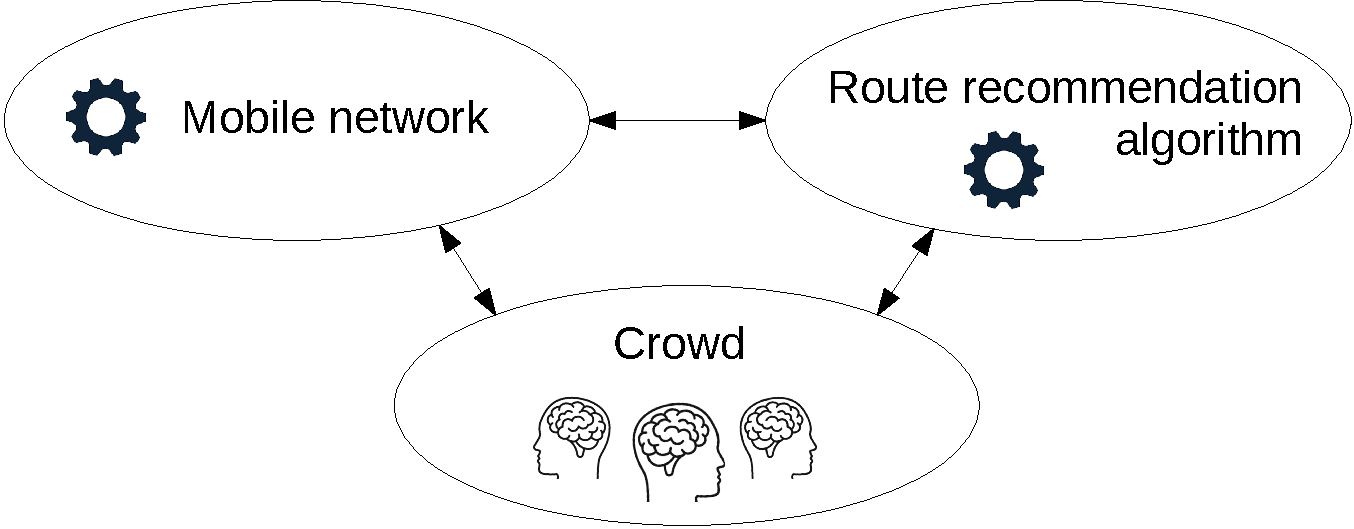
\includegraphics[width=8cm]{../figures/introduction/system.pdf} 
\caption{Components of a crowd guidance system examined in this thesis. I analyze the system from a sociocybernetics perspective, looking at technological and psychological aspects and their interaction.}
\label{fig:techpsycho}
\end{figure}




In step (1), I investigate the suitability of direct communication technology for redirecting mobile crowds. Several studies~\cite{grossglauser-2002-com,bai-2003-com,helgason-2014-com,maccartney-2017-com,chaintreau-2007-cdyn,chancay-2018-com} showed that mobility behavior affects the information dissemination in the mobile network. Crucially, the accuracy of the locomotion model affects the results of the mobile networks simulation~\cite{wischhof-2022b-com}. Many movement models have already been used in network simulations, see the overview~\cite{zhang-2017-com}. Among them are models from the pedestrian dynamics community, such as the Legion Model and the Social Force Model, see~\cite{chancay-2018-com,helgason-2014-com}. So far, only the influence of mobility behavior on the network simulation has been investigated. In a crowd guidance system, however, the mobile network and mobility behavior influence each other bi-directionally: The crowd changes its behavior due to the information disseminated via the mobile network, which, in turn, influences the mobile network.
Such a dynamic system has yet to be investigated. It needs to be clarified how redirection measures affect shadowing and interference, thus, information dissemination in the crowd. My first sub-question therefore asks how reliably redirection information is disseminated in a redirected crowd using direct communication technology, see~\hyperref[reserachquestions]{(RQ-1)}. 



In step (2), I investigate route recommendation algorithms. Meanwhile, numerous guidance approaches have been proposed for crowd management. The algorithms, implemented in the so-called controller, mainly come from engineering. Among them are feedback controllers that aim to affect the locomotion behavior~\cite{kachroo-2010-cdyn, shende-2011-cdyn, shende-2013-cdyn} and controllers trying to influence the decision-making of pedestrians~\cite{zhang-2016-cdyn}. The complexity of these controllers varies greatly from simple On-Off controllers~\cite{gao-2022-cdyn} to more sophisticated methods, such as Model Predictive Control~\cite{menner-2023-cdyn}. 
Unfortunately, most algorithms were developed under unrealistic conditions: It was assumed that the crowd always followed instructions. This is wrong because people may but do not have to follow instructions. Even if they are willing, they may be physically unable or simply not understand what they are supposed to do. I, therefore, find it essential to investigate which algorithms are suitable when not all people follow instructions, see~\hyperref[reserachquestions]{(RQ-2)}.  


In step (3), I investigate how one can improve the compliance of the crowd to follow route recommendations. Studies from communication sciences showed that human behavior can be influenced using message framing, i.e., `presenting logically equivalent options in semantically different ways'~\cite{krishnamurthy-2001-life}. Message framing has been applied in numerous fields like health sciences, marketing, or political communication~\cite{gallagher-2012-life}.  
Techniques from message framing have also been applied to influence crowd behavior: Carter et al.~\cite{carter-2014-life,carter-2015-life} varied the detail of information in a decontamination experiment and found that the crowd complied most when instructions included detailed explanations and instructions. Similar findings have been obtained from studies with individuals~\cite{tormala-2007-life, osman-2018-life}. The communication of information is one factor that can have an impact on behavior. Research from the field of social identity showed that groups and individuals behave differently when group members share a social identity~\cite{reicher-2016-life,carter-2015-life,sivers-2014b-cdyn}.
This can indeed affect the perception of group members~\cite{novelli-2013-life}, and, thus, the decision behavior. Therefore, I want to investigate how message framing can be combined with theory on social identities to find a suitable message design that fosters crowd members to follow route recommendations, see~\hyperref[reserachquestions]{(RQ-3)}.  




I combine methods from computer science, engineering, and the social sciences to answer the main research question and the sub-questions. To investigate the suitability of direct communication in step (1), I model a redirection scenario and conduct a simulation study. I proceed similarly in step (2) to find a suitable route recommendation algorithm. In step (3), an online survey is carried out to assess the effect of message design on route choice. In step (4), I present the complete crowd guidance system, apply it to a real-life use case at the metro station Münchner Freiheit in Munich (Germany), and test it in simulations for which I estimate parameters from the survey data.


\vspace{0.5cm}

\begin{tcolorbox}[title=Proposed methodology for designing a guidance system]
\begin{itemize}
\item[(1)] Test the suitability of direct communication for disseminating route recommendations in a moving crowd $\Rightarrow$~\hyperref[reserachquestions]{RQ-1}. \textit{Method: Modeling \& Simulation}
\item[(2)] Find a suitable route recommendation algorithm $\Rightarrow$~\hyperref[reserachquestions]{RQ-2}. \textit{Method: Modeling \& Simulation}
\item[(3)] Find a message design that convinces crowd members to follow route recommendations $\Rightarrow$~\hyperref[reserachquestions]{RQ-3}.   \textit{Method: Survey}
\item[(4)] Use the findings from (1)-(3) to design and test a proof of concept. $\Rightarrow$~\hyperref[reserachquestions]{RQ}. \textit{Method: Modeling \& Simulation}
\end{itemize}
\end{tcolorbox}

\vspace{0.5cm}




\section{Structure of this work}

The thesis is divided into three main chapters, see Fig.~\ref{fig:leseanleitung}.
Chapter~\ref{sec:state} presents the state of the art on crowd management and approaches for modeling, simulating, and investigating a crowd guidance system. In Chapter~\ref{sec:crownet}, I introduce the novel simulation framework \textit{CrowNet} that was collaboratively developed in the \textit{roVer} research project.
In Chapter~\ref{sec:investigation}, I use this software to investigate my research questions following the proposed methodology. Sections \ref{sec:infoverbreitung}-\ref{sec:reaction} correspond to steps (1)-(3), where I investigate isolated components of a crowd guidance system to answer the research sub-questions. In Section~\ref{sec:realistiscscenario}, I answer the main research question: I propose and test a complete crowd guidance system for a real-life use case at a metro station in Munich (Germany) where football fans need to be guided away from a congested route.


\begin{figure}[hbt!]
\begin{tikzpicture}[thick,scale=0.83, every node/.style={transform shape}]

\node[rectangle,draw=black!60,fill=gray!30,text width=0.9cm] (a1) at (-3.3,0.0)                            {\hyperref[reserachquestions]{RQ-1}};
\node[rectangle,draw=black!60,fill=gray!30,text width=0.9cm] (b1) at (-3.3,1.5)                            {\hyperref[reserachquestions]{RQ-2}};
\node[rectangle,draw=black!60,fill=gray!30,text width=0.9cm] (c1) at (-3.3,3.0)                            {\hyperref[reserachquestions]{RQ-3}};
\node[rectangle,draw=black!60,fill=gray!10,text width=0.7cm] (rq) at (-4.3,10.0)                            {\hyperref[reserachquestions]{RQ}};

\draw [->] (rq) |- (a1);
\draw [->] (rq) |- (b1);
\draw [->] (rq) |- (c1);



\draw[fill=blue!20] (-2.25,-1.5) rectangle ++(4.5,9.7);
\draw[fill=blue!40] (-2,-1.0) rectangle ++(4,5);

\node[rectangle,draw=black!60,fill=white,text width=3.7cm] (d2) at (0,5.0)                            { Co-Simulation and frameworks (\ref{sec:simulationframeworks})};


\node[rectangle,draw=black!60,fill=white,text width=3.7cm] (e2) at (0,6.5)                            { Uncertainty quantifi. and validation (\ref{sec:uq})};




\node[rectangle,draw=black!60,fill=white,text width=3.5cm] (a2) at (0,0.0)                            { Direct communication  (\ref{sec:modelcom})};
\node[rectangle,draw=black!60,fill=white,text width=3.5cm] (b2) at (0,1.5)                            { Route recommendation algorithms  (\ref{sec:modelalg})};
\node[rectangle,draw=black!60,fill=white,text width=3.5cm] (c2) at (0,3.0)                            { Crowd behavior   (\ref{sec:crowdbah}, \ref{sec:modelcrowd})};

\draw [<->,dashed] (a1) -- (a2);
\draw [<->,dashed] (b1) -- (b2);
\draw [<->,dashed] (c1) -- (c2);

\draw[fill=orange!20] (3,-1.5) rectangle ++(4.5,11);
\draw[fill=orange!40] (3.25,-1.0) rectangle ++(4,5.0);

\node[rectangle,draw=black!60,fill=white,text width=3.5cm] (a3) at (5.3,0.0)                            { Module \textit{OMNeT++} (\ref{sec:omnet})};
\node[rectangle,draw=black!60,fill=white,text width=3.5cm] (b3) at (5.3,1.5)                            { Module \textit{flowcontrol } (\ref{sec:flowcontrol})};
\node[rectangle,draw=black!60,fill=white,text width=3.5cm] (c3) at (5.3,3.0)                            { Module \textit{Vadere}  (\ref{sec:vadere})};


\node[rectangle,draw=black!60,fill=white,text width=3.7cm] (d3) at (5.3,6.5)                            { Module \textit{SUQ-controller } (\ref{sec:suqc})};

\node[rectangle,draw=black!60,fill=white,text width=3.7cm] (e3) at (5.3,5.0)                            { Module \textit{crownetutils} (\ref{sec:crownetutils})};


\draw [->] (a2) -- (a3);
\draw [->] (b2) -- (b3);
\draw [->] (c2) -- (c3);
\draw [->] (d3) -- (e3);
\draw [->] (e2) -- (d3);


\draw[fill=purple!20] (8.2,-1.5) rectangle ++(4.6,12.8);

\node[rectangle,draw=black!60,fill=white,text width=4.0cm] (a4) at (10.5,0.0)                            { Information dissemination study (\ref{sec:infoverbreitung})};
\node[rectangle,draw=black!60,fill=white,text width=4.0cm] (b4) at (10.5,1.5)                            { Route algorithm study (\ref{sec:umleitalgorithmen})};
\node[rectangle,draw=black!60,fill=white,text width=4.0cm] (c4) at (10.5,3.0)                            { Survey on message design (\ref{sec:reaction})};
\node[rectangle,draw=black!60,fill=white,text width=4.0cm] (d4) at (10.5,10.0)                            {Crowd guidance system: proof of concept \\ (\ref{sec:realistiscscenario})};
%\draw [black,
    decorate, 
    decoration = {brace,
        raise=-15pt,
        amplitude=5pt}] (8,-4.5) --  (4,-4.5)
node[pos=0.5,black]{Assembling};
\draw [->] (a4) -- (b4);
\draw [->] (b4) -- (c4);
\draw [->] (c4) -- (d4);

\draw [->] (a3) -- (a4);
\draw [->] (b3) -- (b4);
\draw [->] (c3) -| (7.8,1.5);
\draw [->] (c3) -| (7.8,0.0);

\draw [->,dashed] (c2) |- (9.0,3.83) --  (9.0,3.6) ;



\node[isosceles triangle,
    draw,
    fill=black,
    minimum size =0.55cm] (T)at (2.45,7.5){};
    \node[isosceles triangle,
    draw,
    fill=black,
    minimum size =0.55cm] (T)at (7.65,8.8){};
    
\draw [->] (d2) --  (e3);
\draw [<->,dashed] (rq) -- (d4);

\draw [->]  (e3) -- (5.3,4.0) ;


\node[font=\Large] at (0,-1.9){\ref{sec:state} State of the Art};
\node[font=\Large] at (5.2,-1.9){\ref{sec:crownet} Software \textit{CrowNet}};
\node[font=\Large] at (10.5,-1.9){\ref{sec:investigation} Investigation};

\end{tikzpicture}
\caption[Reading instructions]{Reading instructions. The thesis is divided into three main chapters. The arrows indicate how the research question (\hyperref[reserachquestions]{RQ}) and the sub-questions (\hyperref[reserachquestions]{\mbox{RQ-1}}, \hyperref[reserachquestions]{RQ-2}, \hyperref[reserachquestions]{RQ-3}) are related to the individual chapters and sections. }
\label{fig:leseanleitung}
\end{figure}


